\documentclass[11pt,a4paper]{article}
\usepackage[hyperref]{acl2020}
\usepackage{times}
\usepackage{tabularx}
\usepackage{latexsym}
\usepackage{graphicx}
\usepackage{subfig}
\usepackage{commath}
\renewcommand{\UrlFont}{\ttfamily\small}
\newcommand{\spacemanidol}[1]{\textcolor{orange}{\bf \small [#1 --dc]}}
\newcommand{\hayley}[1]{\textcolor{pink}{\bf \small [#1 --h]}}
\setlength\titlebox{5cm}
\newcommand\BibTeX{B\textsc{ib}\TeX}
\usepackage{microtype}
\aclfinalcopy 
\title{LING 573:Document Summarization Project Report}
\author{Daniel Campos, Sicong Huang, Shunjie Wang, Simola Nayak, \and Hayley Luke \\ University of Washington \\ {\tt\{dacamp, huangs33, shunjiew, simnayak, jhluke\}@uw.edu}}
\begin{document}
\maketitle
\begin{abstract}
We design and implement Mockingbird, a topic-focused multi-document extractive summarization system. Building on the LexRank graph algorithm our system uses sentence similarity and topic-sentence bias to produce candidates. Next, the ranked sentences are selected to limit redundancy and stay under 100 words. Our system outperforms the LEAD and MEAD baseline by a fair margin. Future work will focus on forms of text representation and processing along with more complex selection and sorting can improve system performance
\end{abstract}
\section{Introduction}
Topic oriented document clusters like AQUAINT \cite{Graff2002TheAC} and ACQUAINT-2 have been used as a starting point to explore various methods for document summarization. More specifically, these corpuses have been used to study extractive multi-document topic summarization. These corpuses have been the focus of study in TAC(Text Analytics Conference) \cite{Dang2008OverviewOT} summarization shared task. In the formalization of this task give a topic and a set of news wire documents a competitive system should create a high quality summary of the topic using sentences from the documents. Systems are expected to produce summaries up to 100 words and summaries should be coherent and not contain duplication. Once summaries are generated for all the topics being studied, methods are evaluated and compared using the standard ROUGE metric \cite{Lin2004ROUGEAP}.  \\ Our exploratory system, called Mockingbird(MB), is based on the Biased LexRank graph approach \cite{Otterbacher2009BiasedLP}. In this approach, we provide a ranking of all candidate sentences by combining a matrix which represents sentence similarity with a topic and sentence similarity. After a ranking is produced sentences are selected to maximize their lexrank score but minimize duplication of content. Our method relies on word vectors \cite{Mikolov2013DistributedRO} from the spacy library \footnote{https://spacy.io/} to represent sentences and we experiment with the effects of evaluating complete sentences, sentences without stop words, and only the nouns in the sentences. After we have a set of candidate sentences we sort them in reverse chronological order and then realize the content to match the TAC output format. To understand our system performance we compare our systems ROUGE-1 and ROUGE-2 scores when compared to LEAD, and MEAD baselines. Our system across the board performs favorably as we beat the two baselines(MEAD and LEAD). However, our system lags behind the top system from TAC 2010 by a significant margin.
\section{System Overview}
Mockingbird has been designed as a simple end-to-end pipeline with the goal of producing a structure we can continue to tweak and modify to understand the effect of various changes have on downstream performance. The pipeline, represented in \ref{fig:overview}, broadly has 4 steps: document input and processing, content selection, information ordering, content realization. \\
\begin{figure}[h]
  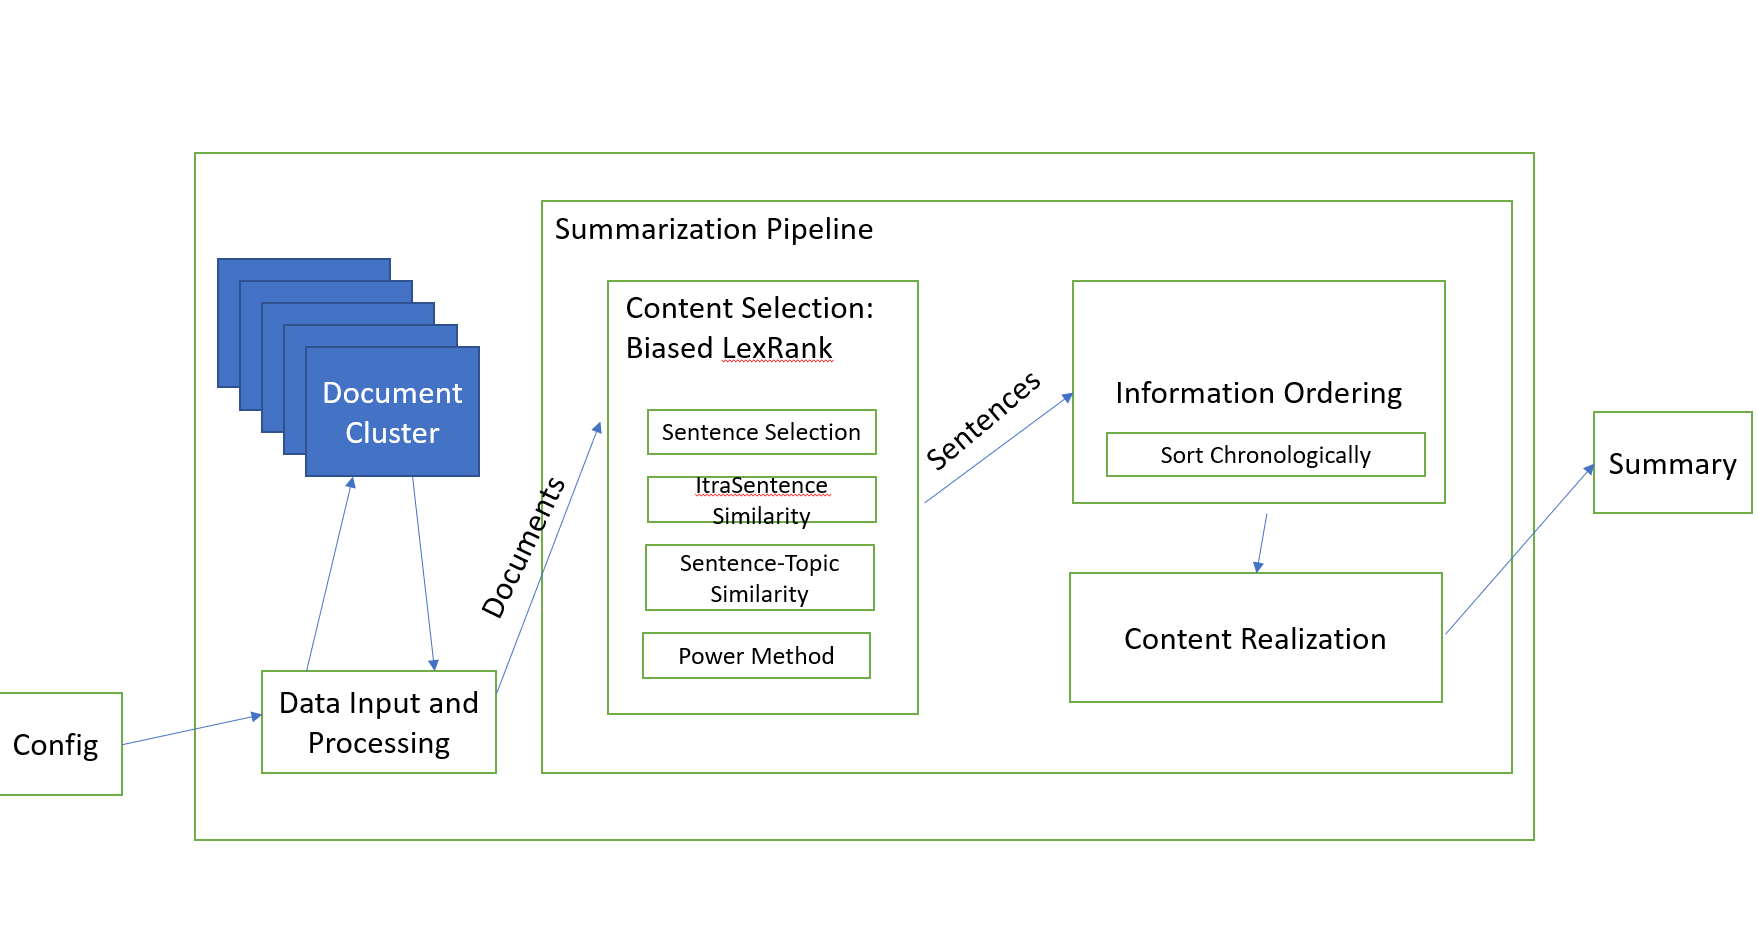
\includegraphics[width=\linewidth]{doc/overview.png}
  \caption{Overview Of Mockingbirds Architecture}
  \label{fig:overview}
\end{figure}
\section{Approach}
In this section we will describe the in detail each of the steps our system takes to summarize topics.
\subsection{Data Input and Processing}
Documents come from the ACQUAINT and ACQUAINT-2 corpus and are a mixture of HTML and XML. The document pipeline takes as an input a configuration file (XML) which details a series of topics and associates the them with a group of document ID's. Using this configuration file, we compile a list of topics, and use the document ID's to determine the path to the relevant corpus file on disk. We then search the file for the information relevant to our specific document ID, and extract the text, the date, and the title. We clean the data, converting the date to a usable format, and stripping excess white space and symbols in the text. Finally, we break the text into sentences using spaCy's sentence tokenization.
\subsection{Content Selection}
Next, there is the content selection pipeline. In this step we consume the structured information from the processing pipeline and produce a candidate set of sentences. Our system selects content using a modified version of the Biased LexRank Graph approach. This method computes a intrasentence and topic-sentence similarity which is used to create a similarity matrix and a bias vector. In this method, each node of the graph represents a sentence and edges between nodes are represented by their intrasentence similarity. This representation allows ranking of sentences to be based on their similarity to the topic and their centrality in the topic document clustering. Our method differs from the original implementation of Lexrank\cite{otterbacher-etal-2005-using} as we leverage word embeddings instead of their tf-idf implementation. \\ 
For each topic we first assemble all sentences in scope of the topic that have at least 4 words. Then, for each sentence, we use spacy to create a vector representation for each sentence. This method leverages the word embeddings known as GloVe \cite{Pennington2014GloveGV} and produces a sentence embedding by averaging the word vectors of each word in the sentence. We experiment with various text normalization methods like stop-word removal and nouns only but broadly the MB pipeline is agnostic. We follow equation \ref{equation:1} to we generate a two dimension matrix representing the cosine similarity between all the sentences related to the topic. Additionally, we create a bias 1d vector which represents the cosine similarity between the topic and each sentence. For inter-sentential cosine similarity, we use a minimum threshold of 0.3 as we find word similarity tends to be higher then tf-idf similarity.\\
We now use sentence embeddings based on \cite{reimers-2019-sentence-bert}
\begin{equation}
\label{equation:1}
similarity(u,v) = cos(u,v) = \frac{u * v}{\norm{u}\norm{v}}
\end{equation}
Using the bias vector and the inter sentence similarity matrix we compute a lexrank for each sentence using the equation \ref{equation:2} where $s$ is a sentence, $q$ is the topic string, $d$ is the weight bias for the topic(set to 0.8), and $S$ represents all sentence in the topic. 
\begin{equation}
   bias(s|q_ =  \frac{cos(s,q)}{\sum_{a \in S} cos(a,q) }
\end{equation}
\begin{equation}
    sentsim(s,S) = \sum_{s_1 \in S} \frac{cos(s,s_1)}{\sum_{s_2 \in S} cos(s_1,s_2) }
\end{equation}
\begin{equation}
\label{equation:2}
lr(s|q) = d * bias(s|q) + (1-d) * sentsim(s,S)
\end{equation}
In our system, we turn our 2d inter-sentential similarity matrix($IS$) and bias vector($BV$) into a matrix $M$ using equation \ref{equation:3}.  Then, we implement the power method, as described in equation \ref{equation:4}, to produce a converged LexRank values for each sentence. As LexRank represents sentence probabilities we initial have a uniform distribution (all sentences are equally likely to show up) and we use the power method until the method converges or an $\epsilon$ of 0.3.
\begin{equation}
\label{equation:3}
M = [d * IS + (1-d) * BV]^T
\end{equation}
\begin{equation}
\label{equation:4}
P_t = M * p_t-1
\end{equation} \\
Once we have assembled sampling probabilities for each sentence we select sentences until we have either used all candidate sentences or reached the target length of 100 words. Sentences are initially ranked by LexRank score and we select candidates that have less than a 0.6 cosine similarity to all other selected sentence. This filter is applied to minimize sentence redundancy. 
\subsection{Information Ordering}
Following content selection we run our information ordering system. We used a basic chronological ordering approach, by sorting our sentence objects by their \texttt{doc\_date} property.\\
\subsection{Content Realization}
Following information ordering we run our content realization system. Currently, this system only formats the text to match the desired file format.
\subsection{Evaluation}
Once all summaries have been created our system moves onto evaluation. 
\section{Results}
To evaluate our system performance we ran our system on the 2010 TAC shared evaluation task. The 2010 TAC task has 43 systems including baselines. The 1st baseline (LEAD), created summaries using the first 100 words from the most recent document. The 2nd baseline was the output of the MEAD summarization system \cite{Radev2003MEADRM}. We have also included system 43 and system 22 as benchmarks because they had the best performance in the shared task(eval and dev set respectively). We evaluate models according to their ROuge-2 and ROuge-1 Recall scores on the devtest portion of the 2010 TAC task. Our system, has three variants indicating various methods of sentence representation. Default uses the sentence average word embeddings without normalization. No Stop words uses sentence average embedding with stop word removed. Nouns uses sentence average embeddings only based on the nouns in the text. \\
Looking at \ref{table:1}, we can see that our system, Mockingbird outperforms the baselines by a fair margin. Our system runs best when removing stop words as this shows a 0.02324 improvement over the default system. While our model is competitive with baselines it is outperformed by a fair margin by system 22, which had the best performance on the devtest set for 2010 TAC. 
\begin{table}[h]
\begin{tabular}{|l|l|l|} \hline
\textbf{System Name} & \textbf{ROUGE-2} & \textbf{ROUGE-1}\\ \hline
LEAD & 0.05376 & - \\ \hline
MEAD & 0.05927 &  -\\ \hline
\textbf{MB}(Default) &  0.05047 & 0.23737 \\ \hline
\textbf{MB}(Nouns) & 0.06704  &  0.32014\\ \hline
\textbf{MB}(No Stop words) & 0.07371 & 0.33193 \\ \hline
System 43 & 0.01154 & -\\ \hline
System 22 & \textbf{0.09574} & - \\ \hline
\end{tabular}
\label{table:1}
\end{table}

\begin{table}[h]
\begin{tabular}{|l|l|l|l|l|l|} \hline
\textbf{Sentence Representation} & \textbf{Dampening} & \textbf{Similarity Threshold} & \textbf{epsilon} & \textbf{ROUGE-1} & \textbf{ROUGE-1}\\ \hline
Transformer & 0.0 & 0.0 & 0.1 & 0.20981 & 0.04281 \\ \hline
Transformer & 0.0 & 0.1 & 0.1 & 0.20154 & 0.04048 \\ \hline
Transformer & 0.0 & 0.2 & 0.1 & 0.20625 & 0.04214 \\ \hline
Transformer & 0.0 & 0.3 & 0.1 & 0.19241 & 0.04359 \\ \hline
Transformer & 0.0 & 0.4 & 0.1 & 0.19431 & 0.05530 \\ \hline
Transformer & 0.0 & 0.5 & 0.1 & 0.19399 & 0.05522 \\ \hline
Transformer & 0.0 & 0.6 & 0.1 & 0.19399 & 0.05522 \\ \hline
Transformer & 0.0 & 0.7 & 0.1 & 0.19399 & 0.05522\\ \hline
Transformer & 0.0 & 0.8 & 0.1 & 0.19399 & 0.05522 \\ \hline
Transformer & 0.0 & 0.9 & 0.1 & 0.19399 & 0.05522 \\ \hline
Transformer & 0.0 & 1.0 & 0.1 & 0.20981 & 0.04281 \\ \hline
Transformer & 0.1 & 0.0 & 0.1 & 0.22791 & 0.05073 \\ \hline
Transformer & 0.2 & 0.0 & 0.1 & 0.23691 & 0.05809 \\ \hline
Transformer & 0.3 & 0.0 & 0.1 & 0.23180 & 0.05667 \\ \hline
Transformer & 0.4 & 0.0 & 0.1 & 0.23151 & 0.05466 \\ \hline
Transformer & 0.5 & 0.0 & 0.1 & 0.22822 & 0.05448 \\ \hline
Transformer & 0.6 & 0.0 & 0.1 & 0.22689 & 0.05438 \\ \hline
Transformer & 0.7 & 0.0 & 0.1 & 0.23141 & 0.05736 \\ \hline
Transformer & 0.8 & 0.0 & 0.1 & 0.22735 & 0.05722 \\ \hline
Transformer & 0.9 & 0.0 & 0.1 & 0.22738 & 0.05781 \\ \hline
Transformer & 1.0 & 0.0 & 0.1 & 0.22607 & 0.05470 \\ \hline
\end{tabular}
\label{table:2}
\end{table}

Similarity threshold 0.4, dampening 0.7
\section{Discussion}
We were surprised how well Mockingbird performed given the simplicity of the system. Given our system design was focused on producing a functional end to end summarization pipeline we were not expecting to beat the MEAD baseline. Given the focus on a functional platform we performed no hyperparameter tuning for all the static values of our lexrank models and thus believe we could improve our system further once we find the optimal values. Moreover, since most of our hyper parameters were based on prior literature and those methodologies rely on tf-idf methodologies we expect our optimal parameters will likely be very different than our current settings.  b We were also pleasantly surprised to find a huge improvement in performance by performing some basic sentence normalization for our sentence representation for vectors. This leads us to believe that there are likely many other sentence normalization approaches that could lead to further gains.  Outside of the content selection model improvements we believe there are likely further gains to be had by implementing less naive strategies in information ordering and content realization. 
\section{Conclusion and Future Work}
Mocking bird(MB) is a topic-based multi-document extractive text summarization that leverages word vectors to select salient sentences. MB is a end to end summarization system that has been implemented in a simple and expandable fashion with the goal of allowing quick tweaks for exploration of model performance. \\
MB uses a modified version of the LexRank similarity graph method which uses inter-sentence similarity and topic sentence similarity to produce a sampling probability for each sentence in a topic. Then, MB select greedily from ranked candidate sentences to reach the 100 word summarization target producing relevant summaries that have little redundancy. \\
MB outperforms the LEAD and MEAD baselines for the 2010 TAC summarization track on the ROUGE-2 scores on the devtest set. MB does best when sentences are pre-process to remove stop words but there is likely substantially more fine tuning that can be done to further improve model scores. MB has had no hyperparameter tuning and thus is likely not performing at its global maxima. \\
In future iterations of MB we will tune our hyperparameters, explore other sentence representations like BERT \cite{Devlin2019BERTPO}, implement more text normalization, and implement more complex and complete information ordering and content realization systems.
Content realization will incorporate sentence parsing in order to facilitate adjectival and adverbial removal. This should help maximize conciseness and allow for more information-dense summaries when required.
\bibliography{acl2020}
\bibliographystyle{acl_natbib}
\end{document}